\documentclass{style/sigchi}

\toappear{\scriptsize Permission to make digital or hard copies of all or part of this work for personal or classroom use is granted without fee provided that copies are not made or distributed for profit or commercial advantage and that copies bear this notice and the full citation on the first page. Copyrights for components of this work owned by others than ACM must be honored. Abstracting with credit is permitted. To copy otherwise, or republish, to post on servers or to redistribute to lists, requires prior specific permission and/or a fee. Request permissions from permissions@acm.org. \\
{\emph{CHI '20, April 25--30, 2020, Honolulu, HI, USA.} } \\
\Copyright~2020 Association of Computing Machinery. \\
ACM ISBN 978-1-4503-6708-0/20/04\ ...\$15.00. \\
http://dx.doi.org/10.1145/3313831.3376624}
% Update the XXXX string to your assigned DOI from ACM.

\clubpenalty=10000
\widowpenalty = 10000

% Arabic page numbers for submission.  Remove this line to eliminate
% page numbers for the camera ready copy
% \pagenumbering{arabic}

% Load basic packages
\usepackage{balance}       % to better equalize the last page
\usepackage{graphics}      % for EPS, load graphicx instead 
\usepackage[T1]{fontenc}   % for umlauts and other diaeresis
\usepackage{txfonts}
\usepackage{mathptmx}
\usepackage[pdflang={en-US},pdftex]{hyperref}
\usepackage{color}
\usepackage[table]{xcolor}
\usepackage{colortbl}
\usepackage{mdwlist}
\usepackage{booktabs}
\usepackage{textcomp}

% Some optional stuff you might like/need.
\usepackage{microtype}        % Improved Tracking and Kerning
% \usepackage[all]{hypcap}    % Fixes bug in hyperref caption linking
\usepackage{ccicons}          % Cite your images correctly!
% \usepackage[utf8]{inputenc} % for a UTF8 editor only

% If you want to use todo notes, marginpars etc. during creation of
% your draft document, you have to enable the "chi_draft" option for
% the document class. To do this, change the very first line to:
% "\documentclass[chi_draft]{sigchi}". You can then place todo notes
% by using the "\todo{...}"  command. Make sure to disable the draft
% option again before submitting your final document.
\usepackage{todonotes}

% Paper metadata (use plain text, for PDF inclusion and later
% re-using, if desired).  Use \emtpyauthor when submitting for review
% so you remain anonymous.
\def\plaintitle{No Explainability without Accountability: An Empirical Study of Explanations and Feedback in Interactive ML}
\def\plainauthor{Alison Smith-Renner, Ron Fan, Melissa Birchfield, Tongshuang Wu, Jordan Boyd-Graber, Dan Weld, Leah Findlater}
%\def\emptyauthor{}
\def\plainkeywords{Interactive machine learning; explainable machine learning}
\def\plaingeneralterms{Documentation, Standardization}

% llt: Define a global style for URLs, rather that the default one
\makeatletter
\def\url@leostyle{%
  \@ifundefined{selectfont}{
    \def\UrlFont{\sf}
  }{
    \def\UrlFont{\small\bf\ttfamily}
  }}
\makeatother
\urlstyle{leo}

% To make various LaTeX processors do the right thing with page size.
\def\pprw{8.5in}
\def\pprh{11in}
\special{papersize=\pprw,\pprh}
\setlength{\paperwidth}{\pprw}
\setlength{\paperheight}{\pprh}
\setlength{\pdfpagewidth}{\pprw}
\setlength{\pdfpageheight}{\pprh}

% Make sure hyperref comes last of your loaded packages, to give it a
% fighting chance of not being over-written, since its job is to
% redefine many LaTeX commands.
\definecolor{linkColor}{RGB}{6,125,233}
\hypersetup{%
  pdftitle={\plaintitle},
% Use \plainauthor for final version.
%  pdfauthor={\plainauthor},
%  pdfauthor={\emptyauthor},
  pdfkeywords={\plainkeywords},
  pdfdisplaydoctitle=true, % For Accessibility
  bookmarksnumbered,
  pdfstartview={FitH},
  colorlinks,
  citecolor=black,
  filecolor=black,
  linkcolor=black,
  urlcolor=linkColor,
  breaklinks=true,
  hypertexnames=false
}

% create a shortcut to typeset table headings
% \newcommand\tabhead[1]{\small\textbf{#1}}


\newcommand{\g}{\, | \,}

\newcommand{\latexfile}[1]{\input{sections/#1}}
\newcommand{\figfile}[1]{figures/#1}

%\newif\ifcomment\commenttrue
\newif\ifcomment\commentfalse

\ifcomment
\newcommand{\pinaforecomment}[3]{\textcolor{#1}{\bf\small [#3 -#2]}}
\else
\newcommand{\pinaforecomment}[3]{}
\fi


\newcommand{\sherry}[1]{\pinaforecomment{blue}{Sherry}{#1}}
\newcommand{\jbg}[1]{\pinaforecomment{green}{JBG}{#1}}
\newcommand{\lkf}[1]{\pinaforecomment{magenta}{LF}{#1}}
\newcommand{\amr}[1]{\pinaforecomment{green}{Alison}{#1}}
%\usepackage{authblk}
%\newcommand{\affiliation}[1]{\thanks{\scriptsize{#1}}}
\newcommand{\revised}[1]{\textcolor{blue}{#1}}
% End of preamble. Here it comes the document.
\begin{document}

\title{\plaintitle}
%\author[1]{\textbf{\large Alison Smith-Renner}}
%\author[2]{\textbf{\large Ron Fan}}
%\author[2]{\textbf{\large Melissa Birchfield}}
%\author[2]{\textbf{\large Tongshuang Wu}}
%\author[1]{\\ \textbf{\large Jordan Boyd-Graber\thanks{Currently at Google Reseach in Zurich}}}
%\author[2]{\textbf{\large Dan Weld}}
%\author[2]{\textbf{\large Leah Findlater}}
%\affil[1]{\affaddr{University of Maryland}, \texttt {amsmit@umd.edu, jbg@umiacs.umd.edu}}

%\affil[2]{\affaddr{University of Washington}, \texttt{rfanhu@gmail.com}, \texttt {\{mbirch2,wtshuang,weld,leahkf\}@uw.edu}}

% (I prefer my personal email here since I basically don't use UW email anymore - Ron)

\numberofauthors{2}
\author{%
Alison Smith-Renner,$^\dag$ Ron Fan,$^\ddag$ Melissa Birchfield,$^\ddag$ Tongshuang Wu,$^\ddag$ \\
Jordan Boyd-Graber,$^\dag$\thanks{Now at
Google Research Z\"urich.}~~Dan Weld,$^\ddag$ and Leah Findlater$^\ddag$
  \alignauthor{
    \affaddr{${}^\dag$University of Maryland}\\
    \affaddr{College Park, MD, USA}\\
    \email{\textttt{amsmit@umd.edu, \\ jbg@umiacs.umd.edu}}}
  \alignauthor{
    \affaddr{${}^\ddag$University of Washington}\\
    \affaddr{Seattle, WA, USA}\\
    \email{rfanhu@gmail.com, \{mbirch2,wtshuang,weld,leahkf\}@uw.edu}}
}


\maketitle

\begin{abstract}
\begin{abstract}

In additon to the traditional task of getting machines to answer
questions, a major research question in question answering is to create interesting,
challenging questions that can help systems learn how to answer
questions and also reveal which systems are the best at answering
questions.
We argue that creating a question answering dataset---and
the ubiquitous leaderboard that goes with it---closely resembles
running a trivia tournament: you write questions, have agents (either
humans or machines) answer the questions, and declare a winner.
However, the research community has ignored the decades of hard-learned
lessons from decades of the trivia community creating vibrant, fair,
and effective question answering competitions.
After detailing problems with existing QA datasets, we outline the key lessons---removing ambiguity, discriminating skill,
and adjudicating disputes---that can transfer to QA research and
how they might be implemented for the QA community.


\end{abstract}

\end{abstract}


% ACM Classfication

\begin{CCSXML}
<ccs2012>
<concept>
<concept_id>10003120.10003121.10003129</concept_id>
<concept_desc>Human-centered computing~Interactive systems and tools</concept_desc>
<concept_significance>500</concept_significance>
</concept>
<concept>
<concept>
<concept_id>10003120.10003121.10011748</concept_id>
<concept_desc>Human-centered computing~Empirical studies in HCI</concept_desc>
<concept_significance>300</concept_significance>
</concept>
<concept>
<concept_id>10010147.10010257</concept_id>
<concept_desc>Computing methodologies~Machine learning</concept_desc>
<concept_significance>300</concept_significance>
</concept>
<concept>
</ccs2012>
\end{CCSXML}

\ccsdesc[300]{Human-centered computing~Interactive systems and tools}
\ccsdesc[300]{Human-centered computing~Empirical studies in HCI}
\ccsdesc[300]{Computing methodologies~Machine learning}

% Author Keywords
\keywords{\plainkeywords}

% Print the classficiation codes
\printccsdesc



% intro

\section{Orthogonal Cross-Lingual Mappings}\label{sec:intro}

Cross-lingual word embedding (\abr{clwe}) models map words from
multiple languages to a shared vector space, where words with similar
meanings are close, regardless of language.
\abr{clwe} is widely used in multilingual natural language
processing~\citep{klementiev-12,guo-15,zhang-16}.
Recent \abr{clwe} methods~\citep{ruder-17,glavas-19} independently train two
monolingual embeddings on large monolingual corpora and then align them
with a linear transformation.
Previous work argues that these transformations should be
\emph{orthogonal}~\citep{xing-15,smith-17,artetxe-16}: for any two words, the
dot product of their representations is the same as the dot product with the
transformation.
This preserves similarities and substructure of the original monolingual word
embedding but enriches the embeddings with multilingual connections between
languages.

\begin{figure*}[!t]
  \centering
  \includegraphics[width=.8\linewidth]{\figfile{girl.pdf}}
  \caption{The most similar Japanese words for \ja{少女} (sh\={o}jo ``girl'')
  and English words for ``girl'', measured by cosine similarity on Wikipedia
  fastText vectors, before (left) and after (right) \name{}.
  In the original embedding spaces, ``boy'' is the nearest neighbor for both
  languages but with a very different cosine similarity, and ``cat'' in English
  is not close to ``girl'': both violate the isomorphism assumed by an
  orthogonal transformation for cross-lingual representations.
  \name{} replaces \ja{猫} (neko ``cat'') with the more
  relevant \ja{美少女} (bish\={o}jo ``pretty girl'') and brings cosine similarities 
  closer.}
  \label{fig:example}
\end{figure*}

Thus, many state-of-the-art mapping-based \abr{clwe} methods impose an
orthogonal
constraint~\citep{artetxe-17,conneau-18,alvarez-18,artetxe-18b,ruder-18,alvarez-19}.
The success of orthogonal methods relies on the assumption that embedding spaces
are isomorphic; i.e., they have the same inner-product structures across
languages, but this does not hold for all
languages~\citep{sogaard-18,fujinuma-19}.
For example, English and Japanese fastText vectors~\citep{bojanowski-17} have
different substructures around ``girl'' (Figure~\ref{fig:example} left).
As a result, orthogonal mapping fails on some languages---when
\citet{hoshen-18} align fastText embeddings with orthogonal mappings, they
report 81\% English--Spanish word translation accuracy but only 2\% for the
more distant English--Japanese.

While recent work challenges the orthogonal
assumption~\citep{doval-18,joulin-18,jawanpuria-19}, we focus on whether simple
preprocessing techniques can \emph{improve the suitability of orthogonal
models}.
Our iterative method normalizes monolingual embeddings to make their structures
more similar (Figure~\ref{fig:example}), which improves subsequent
alignment.

Our method is motivated by two desired properties of monolingual embeddings
that support orthogonal alignment:
\begin{enumerate*}
\item Every word vector has the same length.
\item Each language's mean has the same length.
\end{enumerate*}
Standard preprocessing such as dimension-wise mean centering and length
normalization~\cite{artetxe-16} do not meet the two requirements at
the same time.
%
Our analysis leads to \emph{\name{}}, an alternating projection
algorithm that normalizes any word embedding to provably satisfy both
conditions.
%
After normalizing the monolingual embeddings, we then apply
mapping-based \abr{clwe} algorithms on the transformed embeddings.

We empirically validate our theory by combining \name{} with three
mapping-based \abr{clwe} methods.
%
\name{} improves word translation accuracy on a dictionary induction benchmark
across thirty-nine language pairs.

\section{Related Work}
%This paper explores the relationship between explanations and feedback in ML. First 
We review related work in interactive and explainable ML, separately, and then describe prior studies on their relationship. 

%Interactive ML
\subsection{Interactive Machine Learning}

Compared to classical supervised ML's focus on static labels and
datasets, interactive machine learning (IML) trains a model through rapid end \emph{user}
interaction~\cite{Amershi2014PowerLearning}.
%
IML commonly produces higher quality models~\cite{Settles2010ActiveSurvey, Raghavan2006ActiveInstances}, personalized recommendations~\cite{Amershi2012Regroup:Networks, Gowacka2013DirectingKeywords} or
models that are better aligned with users'
understanding~\cite{Hu2014InteractiveModeling,
Lee2012IVisClustering:Modeling}.
%
However, user feedback can have negative effects: decreased system 
performance~\cite{Ahn2007OpenHarm, Wu2019LocalAnalysis} or 
inconsistent mental models~\cite{Bansal2019UpdatesTradeoff}.

This ``human-in-the-loop'' approach has been applied across machine
learning, including in supervised
ML~\cite{Fails2003InteractiveLearning, Settles2010ActiveSurvey},
unsupervised ML~\cite{Balcan2008ClusteringFeedback}, and reinforcement
learning~\cite{Knox2012ReinforcementTasks,
Saunders2018TrialIntervention}.
%
We focus on supervised ML as it provides intuitive mechanisms for non-ML expert, end user
feedback, such as providing training
examples~\cite{Fiebrink2009ALearning},
preferences~\cite{Resnick1994GroupLens:Netnews}, or by
reacting to model predictions with instance-level (i.e., correcting or
confirming predictions~\cite{Fails2003InteractiveLearning,
Culotta2006CorrectiveExtraction}) or feature-level feedback (i.e.,
denoting features indicative of each
class~\cite{Settles2011ClosingInstances,
Kulesza2015PrinciplesLearning, Raghavan2006ActiveInstances}). Our focus on end users providing feedback, and in particular feature-level feedback aligns with ``Machine Teaching'', where non-ML experts build models from more than just labeled data~\cite{Wall2019UsingTeaching}.

%
%Our studies use a text classification system that supports instance
%and feature-level feedback, similar to
%Settles~\cite{Settles2011ClosingInstances} and Kulesza et
%al.~\cite{Kulesza2015PrinciplesLearning}.

\subsection{Explainable Machine Learning}
% Explainable Machine Learning
% in general
Explainability (or intelligibility) in ML has received growing
attention as ML models take on more important responsibilities in
society.
%
More complex models are often more accurate.
%
Thus, intelligibility research both develops global explanations, such as more transparent
models~\cite{Caruana2015IntelligibleReadmission,Alvarez-Melis2018TowardsNetworks,
Lage2018Human-in-the-loopPrior, Si2013LearningDetection} or black-box explanations~\cite{Lakkaraju2019FaithfulModels}, and local explanations of individual algorithm decisions, which can include
input evidence~\cite{Lei2016RationalizingPredictions,
Feng2019WhatPlay},
localizations~\cite{Selvaraju2017Grad-CAM:Localization,
Park2017AttentiveAbstract}, natural language
explanations~\cite{Camburu2018E-SNLI:Explanations,
Ehsan2019AutomatedPerceptions, Gkatzia2016NaturalInformation}, or
local approximations~\cite{Ribeiro2016WhyClassifier}.
%
We focus on local explanations (i.e., highlighting
important words).

Explanations can support
fairness and bias assessments~\cite{Dodge2019ExplainingJudgment}, improve perceived understanding~\cite{Kocielnik2019WillSystems},
promote system
acceptance~\cite{Herlocker2000ExplainingRecommendations}, engender
trust~\cite{Pu2006TrustInterfaces}, and convince users to accept
recommendations~\cite{Cramer2008TheRecommender}. However, explanations can decrease users' perceptions when algorithmic limitations or uncertainty
are portrayed~\cite{Cai2019TheInterface,
Stowers2017InsightsUncertainty, Lim2011InvestigatingApplications}.
%
Explanations can have other negative effects, such as over-reliance~\cite{Stumpf2016ExplanationsSystems} or inability to detect
mistakes~\cite{Poursabzi-Sangdeh2018ManipulatingInterpretability}.
%
ML-based systems can set expectations by exposing accuracy~\cite{Yin2019UnderstandingModels} or anticipated system mistakes~\cite{Kocielnik2019WillSystems}. This work explores whether such insight in turn increases users desire to fix mistakes and improve systems.
%
%This work explores how explanations with or without the opportunity
%for feedback impact user satisfaction (frustration, trust, acceptance)
%and how users expect these models to change.

Prior work explores the effect of explanations on mental models, in
particular on \textit{predictability}, or the users' ability to
predict model
behavior~\cite{Poursabzi-Sangdeh2018ManipulatingInterpretability,
Chandrasekaran2019DoHuman, Bunt2007UnderstandingCustomization},
finding conflicting results. Explanations improved predictability for apartment pricing~\cite{Poursabzi-Sangdeh2018ManipulatingInterpretability} and GUI customization~\cite{Bunt2007UnderstandingCustomization}, but did not have an effect for a visual question answering~\cite{Chandrasekaran2019DoHuman}.
%
This discrepancy could be because that users expected the ML model to change and therefore were less successful at predicting future model behavior.
%
Our studies measure expected change by asking
users whether they think the system they evaluated will have higher, similar, or lower accuracy on new data.

\subsection{Relationship of Explainability and Interactivity in ML}
% explainable + interactive

Users need to understand how models work~\cite{Fiebrink2009ALearning, Amershi2010ExaminingLearning, Kulesza2012TellAgent} to best fix
them, and how models are explained changes user
feedback~\cite{Rosenthal2010TowardsData,
Kulesza2015PrinciplesLearning}.
%
%Rosenthal and Dey's study~\cite{Rosenthal2010TowardsData} suggest that presenting a system's prediction and low-level context (e.g., an email has
%keywords ``A'' and ``B'') helps users give effective feedback.
%
Kulesza et al.~\cite{Kulesza2015PrinciplesLearning} introduced EluciDebug, based on the concept of
``explanatory debugging'', in which a classifier
explains binary predictions to users in the form of important input
words and proportion of the data labeled as each class.
%
Users in turn inform the classifier by correcting the prediction---\textit{instance feedback}---or saying which words are important for each
class---\textit{feature feedback}.
%
Users both better understood and corrected  EluciDebug's mistakes compared to a system without explanations or feature-level feedback.
%
%, yet for simplicity, we show and support interaction with only the
%word features within each example.
While these studies tell us that explanations foster better feedback,
prior work has not investigated how user perceptions---such as
frustration and trust---are shaped by the presence or (sometimes more
importantly) absence of IML feedback and explanations. Therefore, we address this using a similar data set, task, explanation, and feedback mechanisms.





\section{Comparative evaluation of \hltm{} modeling approaches}

For this study, crowd workers interacted with a topic model to organize documents using one of three contrasting
\hltm{} approaches based on \lda~\cite{blei-03}. The approaches support the same set of nine refinement operations (e.g., merging topics and removing words or documents from topics), and differed only in implementation details, as these criteria affect model attributes, such as adherence, instability, quality, and latency.

This study used a between-subjects experimental design with a single factor (\textit{Modeling Approach}): informed priors using Gibbs sampling
(\textit{info-gibbs}), informed priors using variational inference~(\textit{info-vb}), and constraints using Gibbs sampling
(\textit{const-gibbs}). 

The goal of this study was to explore how users perceive and interact with transparent systems with varied attributes: adherence, instability, latency, and quality. This study explored specifically: 
(RQ1) How do users perceive instability and adherence across the three \hltm{} approaches? 
(RQ2) How does user experience vary given these differing attributes? 
(RQ3) How do users behave with the three \hltm{} approaches?

\subsection{Modeling Approaches}

We implemented three \hltm{} systems, based on \lda{}, following modeling approaches
proposed in prior work~\citep{kumar-19}. These modeling
approaches differ in how user input (e.g., added words) is conveyed to the model---informed priors~\cite{Smith2018ClosingSystem} or constraints~\cite{yang-15}---and inference strategies---variational inference~\cite{blei-03} or Gibbs sampling~\cite{griffiths-04}.

While other topic modeling approaches exist~\cite{Larochelle2012AModel,Hofmann1999ProbabilisticIndexing}, we chose these  \lda-based variants because they support the same user-preferred refinement set. For example, ``anchor words''-variants~\cite{Lund2017TandemModeling} also generate topics, but cannot support word-level operations like adding words. Also, these approaches may differ by the attributes of interest. For example, prior work asserts that informed priors better \textit{adhere} to refinement operations~\cite{kumar-19}, and Gibbs sampling-based methods
can yield more coherent topics~\cite{Nguyen2015ImprovingModeling}.
Also, Gibbs sampling and variational inference have different convergence rates~\cite{asuncion-09b}. While Gibbs sampling is often preferred for small datasets and interactive settings because of its low latency, variational inference can scale to millions of documents~\cite{hoffman-10,Zhai2012MrMapReduce}. 
Our setting allows a focused, task-center comparison (Section~\ref{sec:calculated-differences}).

For \textit{info-gibbs} and \textit{const-gibbs}, we trained initial \lda{}
models with $300$ Gibbs sampling iterations and default Mallet toolkit\footnote{\url{http://mallet.cs.umass.edu/}} hyperparameters ($\alpha=0.1; \beta=0.01$)
and, for \textit{info-vb}, $30$ \abr{em} iterations.
For each subsequent update during the task, we applied the refinement
and ran inference.


\subsection{Refinement Implementations}

For each of the three \hltm{} modeling approaches, we implemented the same nine
refinement operations preferred by users in prior
work~\cite{Lee2017TheModels,Musialek2016UsingApproach,Smith2018ClosingSystem}. These include four topic-level refinements: \textbf{add word, change word order, remove word, remove document} and five model-level refinements: \textbf{merge topics, split topic, create topic, delete topic, add to stop words}. 

For \textbf{remove word, add word, remove document, merge topics, split
  topic, change word order} and \textbf{create topic}, we
applied the refinements following the implementation proposed by
\etalcite{Kumar}{kumar-19}.
For \textbf{add to stop words}, to add a word $w$ to the stop words list, we excluded $w$ from
the model vocabulary. For \textbf{delete topic}, to delete a specified topic $t$, in all three
models, we first forgot all latent topic assignment which were
assigned to $t$, and then reduced the number of topics by one.

After refinements were applied, we ran inference for $N$ iterations to
limit latency (rather than running inference until convergence).
Moreover, all refinements have different levels of complexity, meaning
the models converge faster for certain refinements than others.  For
example, \textbf{add to stop words} is a simpler refinement than
\textbf{create topic}, and hence requires fewer iterations to
converge.  For each refinement, we empirically fine-tuned $N$ on
$9000$ tweets randomly selected from a different
dataset.\footnote{\url{https://www.kaggle.com/kazanova/sentiment140/}}
In particular, to fine-tune $N$ for a refinement, we randomly applied
a refinement multiple times and observed how fast the model converged.
For \textit{info-gibbs} and \textit{const-gibbs}, $N$ ranged from one
for \textbf{add to stop words} to $20$ for \textbf{create topic}. For
\textit{info-vb}, $N$ varied from one for \textbf{add to stop words}
to four for \textbf{create topic}.

\subsection{Dataset}
For the study we used the Twitter Airline Sentiment Dataset, which
includes tweets directed at various common airlines (e.g., United,
Southwest Airlines, Jet Blue) and manually tagged by sentiment
(positive, negative,
neutral).\footnote{https://www.kaggle.com/crowdflower/twitter-airline-sentiment}
We produced initial topic models of
$10$ topics from only the $9,178$ negative sentiment tweets, as these
reflect a distinct set of complaints regarding air
travel. 

        
\begin{figure*}[t]
  \centering
  
  \includegraphics[width=0.75\textwidth]{\figfile{ui5}}
  \caption{\hltm{} interface. Initial model (top)
    represented as a list of topics, each displayed with topic \abr{id}
    and three most probable words. Selecting a topic reveals the top 20 words and top 20 documents.  
    Participants refined the model, including merging topics by
    clicking ``merge'' next to the topic and selecting
    additional topics with which to merge (bottom left), and splitting
    topics by clicking ``split'' next to the topic and
    dragging to separate words into sub-topics (bottom right).  }
  \label{fig:ui}
\end{figure*}

\subsection{Task Interface}

The \hltm{} task user interface was the same for all three modeling
approaches (Figure~\ref{fig:ui}).
The topics are listed on the left, each initially represented by a generic topic label (e.g.,
``Topic 1'') and the three most probable words for the topic. 
The selected topic is on the right, which displays
the top 20 topic words and the top 20 topic documents. Documents
are ordered by their probability for the topic $t$ given the document
$d$, or $p(t \g d)$.
Each word, $w$, is ordered and sized by its probability for the topic
$t$, or $p(w \g t)$; this simple word list representation provides
a quick understanding of the
topic~\cite{Alexander2016AssessingGist-Forming,Smith2017EvaluatingLabels}. Hovering
or clicking on topic words highlights the word in the displayed
document snippets. Participants can click the pencil icon to rename the topic
labels to be more descriptive.

Participants can explore and update the model using the set of nine
refinement operations:
click ``x'' next to words or documents to remove them, select and drag
words to re-order them, type new words into the input box and press
``enter'' to add them, select a word and click ``remove selected word
from all topics'' to add it to the stop words list, click ``delete
topic'' to remove the selected topic, or click ``create a new topic'',
``split'', or ``merge'' (in the topic list) to enter into create,
split, or merge modes, respectively (Figure~\ref{fig:ui}).
Each refinement is immediately saved and the model is updated. After
updates, participants can \textit{undo} to revert models to prior states.

\subsection{Participants}
We recruited $100$ participants ($32$ male and $68$ female) on the
Upwork platform.\footnote{https://www.upwork.com/} Participants were
  required to have a 90\% or higher job success score and be native or
  bilingual English speakers. 
  We designed the task to take approximately 60 minutes and paid participants $20$ \abr{usd}. We used Upwork instead of other common crowdworker platforms (e.g., Mechanical Turk), to recruit more motivated participants; participants were paid a higher rate and could always contact one of the researchers in case of questions. 
  
Participants varied in age ($<19$: four, $20-29$: $46$, $30-39$: $23$,
$40-49$: $13$, $50-59$: seven, $>60$: eight), education (college
degree: $49$, graduate degree: $29$, some college: $17$, high school
or \abr{ged}: $5$), and background ($12$ in English or writing, seven
in education, and five in business).

To understand participants' prior exposure to topic models and machine learning, as this could affect our results, study participants rated prior experience with statistical topic modeling and machine learning, respectively.
Participants varied for prior
experience (rated on a scale from one to five) with topic models (``none'' (one): $44$, two: $25$, three: $18$, four: seven, ``significant'' (five): six) and machine learning (``none'' (one): $44$, two: $19$, three: $19$, four: nine, ``significant'' (five): seven). 

\subsection{Procedure}
\label{sec:procedure}
Each participant was randomly assigned to one of the three
modeling approaches and all used the same \hltm{}
user interface (Figure~\ref{fig:ui}). 
Each user got a unique starting model from a pool of $50$ pre-trained initial \lda{} models with $10$
topics for each of the three \hltm{} modeling approaches. 
Given the assigned approach, we randomly selected an initial topic model from the pool
of pre-trained models and then removed the selected model from the
pool. 
The study began with a tutorial, which introduced participants to topic modeling, relevant terminology, and the task interface. The tutorial also required participants to experiment with each of the nine refinement operations. 
After the tutorial, participants were given the following task instructions: 
\begin{quote}
    ``Imagine you have been asked to write a travel blog post about the common complaints that travelers have when flying. The system has gathered 9000 tweets of people complaining about their air travel experience directed at various popular airlines and has generated an initial set of 10 topics to organize these air travel complaint tweets. Use the tool to improve these topics, so that you can write a blog post about common air travel complaints with a few example tweets from each. You do not need to write the actual blog post as part of this task.''
\end{quote}

Participants were then asked to spend
$30$ minutes interacting with the model and to click the ``finish task'' button when they
were happy with the organization they had achieved. 
The interface required participants to spend at least $20$ and no more
than $45$ minutes on the task. 
The task goal and time elapsed were denoted in the interface
(Figure~\ref{fig:ui}).

After the task, participants completed a survey containing closed- and
open-ended questions on their perceptions and experience with the
system (Table~\ref{tab:subjective_measures}) and which refinements
they felt were the most and least useful, with follow up ``why''
questions. Participants also responded to whether they noticed any
unexpected behavior while using the tool and what they liked and did
not like about using the tool for the task.

\begin{table}[t!]
    \caption{Seven-point rating scale statements for nine subjective measures. All are on a scale from ``strongly disagree'' to ``strongly agree'' aside from satisfaction, which is on a scale from ``not at all'' to ``very'' and improvement, which is on a scale from ``much worse'' to ``much better.''}
    \scriptsize
    \begin{center}
       \begin{tabular}{l p{5cm}}
        \toprule
        Measure & Statement \\
        \midrule
        frustration & ``Using this tool to perform the task was frustrating''\\
        trust & ``I trusted that the tool would update the organization of tweets well''\\
        task ease & ``It was easy to use this tool to perform the task''\\
        confidence & ``I was confident in my specified changes to the tool''\\
        final model satisfaction & ``How satisfied are you with the final organization of the tweets into categories of air travel complaints?''\\
        model improvement & ``How do you think the final organization compares to the initial organization of tweets?''\\
        low latency & ``After my changes, the tool updated quickly''\\
        adherence (overall) & ``The tool made the changes I asked it to make''\\
        instability & ``The tool made unexpected changes beyond what I asked it to make''\\
        \bottomrule
    \end{tabular}
    \end{center}
    \label{tab:subjective_measures}
\end{table}

\subsection{Measures}
We report on nine overall subjective measures, collected using seven-point rating scales (Table~\ref{tab:subjective_measures}): four \textit{user experience} measures (frustration, trust, task ease, confidence) and five \textit{user perception} measures (perceived adherence, perceived instability, perceived latency, final model satisfaction, and perceived improvement). We also report on subjective per-refinement adherence, collected using seven-point rating scales (strongly disagree to strongly agree) for nine statements of the form, ``the system incorporated the [refinement] operation as I asked it to.'' These statements also included a ``did not use operation'' option.

We also report on quantitative measures of the system attributes: adherence, instability, latency, and quality (initial, final, and improved). 
To compute \textit{adherence} for each of the nine refinements we use the metrics provided by~\etalcite{Kumar}{kumar-19}:
\begin{itemize}
    \item \textbf{add word}, \textbf{remove word}, and \textbf{change word order}: treat the topic as a ranked word list, and then take the ratio of the actual rank change (where the added, removed, or reordered word is in the updated model) and the expected rank change.
    \item \textbf{remove document}: compute similarly to \textbf{remove word}, except treat the topic as a ranked document list.
    \item \textbf{create topic}: compute the ratio of the number of seed words in the created topic out of the total number provided.
    \item \textbf{split topic}: compute the average adherence of the parent and child topic, using the adherence measure for \textbf{create topic}.
    \item \textbf{merge topics}: compute the ratio of the number of the words in the merged topic that came from either of the parent topics over the total number of words shown to the user.
    \item \textbf{add to stop words} and \textbf{delete topic}: these refinements are deterministic, and therefore always have a perfect adherence score.
\end{itemize}
Adherence is measured on a range from $0.0$, meaning the system ignores the user's input, to
$1.0$, meaning the system does exactly as the user asks.
  The exception is adherence to
\textbf{change word order}, which ranged from $-\infty$ to $\infty$, and where a
negative adherence value means the system did the opposite of what the
user asked. For example, if a user moves a word up two positions, but it is instead moved down one, the adherence would be $-.5$. 
Overall adherence is computed as the average adherence score over all refinements applied by the user.


To estimate the \textit{instability} caused by a refinement, we use a modified topic-term stability metric~\cite{belford2018stability}. We first compute the difference between each topic as $1.0$ minus the overlap coefficient~\cite{M.K2016AMining} between the top 20 words of the topic, before and after the refinement. Instability is then measured as the average difference between each topic excluding the refined topic(s). Put simply, we compute what percentage of topic words are removed after an update for the untouched topics. Instability is scored from $0.0$ (all topics the same) to $1.0$ (all topics completely different). 
\textit{Latency} is the time the model takes to incorporate each refinement. 
We also computed each participants' initial and final topic model quality as the models' average
\npmi{}-based topic coherence~\cite{Lau2014MachineQuality}; \textit{quality} is thus the difference (i.e., improvement or degradation) from initial to final model quality.\footnote{Automatic coherence metrics require an external reference corpus for \npmi{} computation; as in prior work, we use Wikipedia.  As the Twitter-based topics included many words not found in the
Wikipedia reference corpus, their overall topic coherence scores were
relatively low, but are still useful for \emph{relative} comparison.} We additionally logged all interactions with the system including how
many and which refinements participants applied.

\subsection{Data and Analysis}
\label{sec:analysis}
We disqualified five of the $100$ participants because they made an outlying number of survey
response ``mistakes'' on per-refinement adherence statements. We considered a response to be a ``mistake'' if
the participant said they had used a refinement for the task when they had not, or vice versa, and
used an interquartile range (IQR) approach to determine outliers based on the count of mistakes~\cite{Tukey1977ExploratorySection}: the median
number of mistakes was two, and the upper
quartile bound for outliers ($Q3 + 1.5IQR$) was five (out of nine
possible mistakes). Removing outliers above this bound resulted in $95$ participants in our final dataset: $31$ in the \textit{info-gibbs} condition, $33$ in the
\textit{const-gibbs} condition, and $31$ in the \textit{info-vb}
condition.  

For quantitative analysis, we used separate Kruskal Wallis tests to determine significance across the conditions for each of the subjective rating responses and the quantitative measures. For qualitative analysis, we followed a thematic
approach~\cite{Braun2006UsingPsychology}, and coded the open-ended responses related to what participants found unexpected, liked and did not like, and which refinements they found were most and least useful. Two annotators independently coded a random subset of 20 of the 95 responses for each of the statements regarding what was \textit{unexpected}, what participants \textit{liked}, and what they \textit{disliked}; agreement was scored using Cohen's $\kappa$: $\kappa=.93$ for \textit{unexpected} responses, $\kappa=.88$ for \textit{liked} responses, and $\kappa=.89$ for \textit{disliked} responses.




\subsection{Results}
Figures~\ref{fig:study1measures} and \ref{fig:study1exp} show the rating scale responses for the seven main subjective measures by condition. 
%
Participants expected the model to improve, and they expected more improvement with feedback. Participants also thought the ability to provide feedback was important. 
%
Explanations hurt subjective satisfaction (frustration, trust, and acceptance ratings), while feedback helped.
%
Participants were commonly frustrated by the model's low quality, and this was accentuated by explanations. 

To judge user comfort with the task and dataset, we asked participants to tell us (i.e., the researchers \dots not the model) whether they thought each email was about hockey, baseball, or whether they were unsure.
%
Participants did well: 91\% of the 3,580 answers reported to us were correct, while 8\% were ``not sure'' and only 1\% were incorrect. In the following sections, we provide detailed results regarding satisfaction, expectations, perceptions, feedback quality, and users' desire to provide feedback.

\begin{figure}[t]
    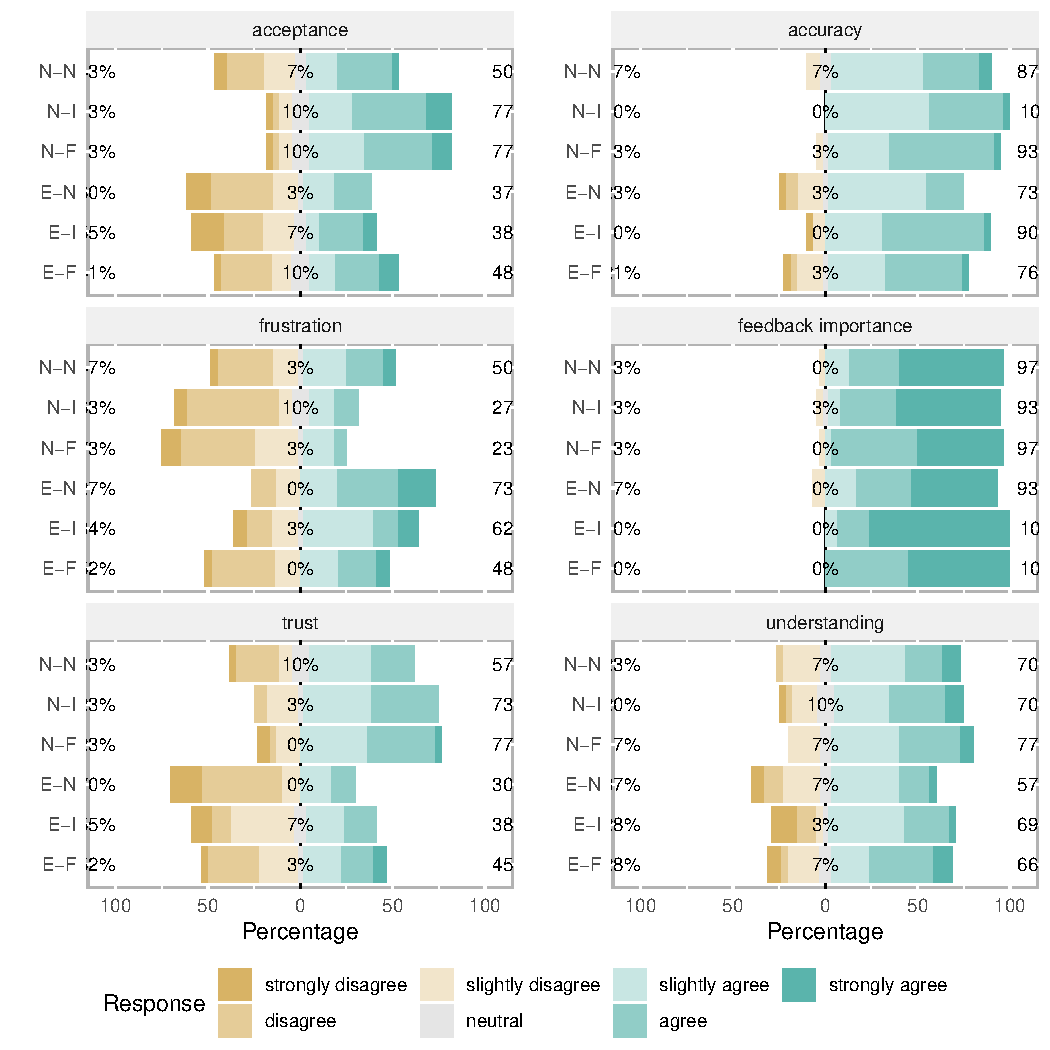
\includegraphics[width=\linewidth]{2020_chi_explanation/figures/study1-measures}
    \caption{Study~1 seven-point rating scale responses for the main subjective measures (except expected change) from ``strongly disagree'' to
``strongly agree''. Responses reported by condition. For each measure,
no explanation (N-) conditions are on the top (-N is with no feedback, -I
is with instance-level feedback, and -F is with feature-level feedback) and
feature explanation (E-) conditions are below Feedback (-I, -F) positively,
and explanation (E-) negatively impact satisfaction measures (left).}
\label{fig:study1measures}
\end{figure}

\subsubsection{User Satisfaction}
% four points: frustration measure, why frustrated, trust, acceptance
Participants were neutral on average, but with high variability across conditions, for each of the user satisfaction measures: frustration ($M=3.9$ of 7, $SD=1.8$), trust ($M=4.1, SD=1.7$), and whether they would use the system (acceptance) ($M=4.3, SD=1.9$).
%
Feedback significantly improved satisfaction, but explanations hampered it. Open-ended responses suggested that the low model quality---highlighted by explanations---frustrated participants.

\textbf{Explanations increased frustration, while support for feedback reduced it}. 
%
Participants who received explanations were more frustrated than those who did not; this difference was significant (main effect of \textit{Explanation}: $F_{1, 172}=20.05, p < .001$). \textit{Feedback} also significantly impacted frustration (main effect: $F_{2, 172}=7.92, p < .001$). Posthoc pairwise comparisons showed that no feedback resulted in significantly higher frustration than instance-level and feature-level feedback (both comparisons $p<.05$); this supports \textbf{H1.1} for frustration, which stated that feedback would reduce frustration. The interaction between \textit{Explanation} and \textit{Feedback} was not significant ($F_{2, 172}=.06, p=.094$); thus, \textbf{H1.2} is only partially supported by the main effect of \textit{Feedback}. 

% why frustrated
\textbf{Many participants were frustrated by low quality, which was highlighted by explanations}.
%
We coded participants' open-ended reasons for their frustration ratings, resulting in six codes. Participants felt the model was: ``not good enough'' ($40\%$ of the 178), or ``good enough'' ($27\%$), would help ``save time'' ($13\%$), would ``require user review'' of the decisions ($11\%$), is ``able to improve'' ($3\%$), or ``other'' reasons ($6\%$).

Confirming the rating scale data, more participants with explanations ($81\%$ of 89) thought the model was ``not good enough'' compared to those who did not get explanations (only $26\%$ of 89).
%
Participants who got explanations (E-) often expressed their frustration in terms of the important words, e.g., \textit{``I don't think it highlighted the best words in many cases''} (LP3, E-I), while those who did not see explanations (N-) were more likely to comment on the model's shortcomings in terms of accuracy, \textit{``it made too many mistakes''} (LP175, N-N). 
%
%``Requires user review'' was a similar concern mentioned by 11\% of all 179 participants, such as \textit{``it would take longer to do my job because I would have to check for accuracy''} (LP151, E-I).

Less frustrated participants felt the model was ``good enough'' or would ``save time'', saying, for example, %\textit{``this model appears to sort the emails with an acceptable degree of accuracy''} (LP52 N-F) and, 
\textit{``It would be much easier than sorting through them myself''} LP132 (E-N).
%Demonstrating lower frustration, 27\% of all participants felt the model was ``good enough,'' such as, \textit{``this model appears to sort the emails with an acceptable degree of accuracy''} (LP52, N-F), and 13\% thought that it would ``save time,'' such as, \textit{``It would be much easier than sorting through them myself''} (LP132, E-N).

% trust measure
\textbf{Trust and acceptance were reduced by explanations and increased by feedback}.
%
Reflecting the frustration findings, trust was significantly impacted by \textit{Explanation} ($F_{1, 172}=14.57, p < .001$); participants who received explanations trusted the model less those who did not. There was also a significant main effect of \textit{Feedback} on trust ($F_{2, 172}=4.27, p = .015$). Posthoc pairwise comparisons showed that both instance- and feature-level feedback increased trust compared to none (both comparisons $p<.05$). The \textit{Explanation} $\times$ \textit{Feedback} interaction was not significant ($F_{2, 172}=.15, p=.863$).

Similarly, \textit{Explanation} significantly impacted acceptance ($F_{1, 172}=19.49, p < .001$), where participants who saw explanations accepted the model less than those who did not. 
\textit{Feedback} also significantly impacted acceptance ($F_{2, 172}=3.76, p=.025$). Posthoc pairwise comparisons showed that feature-level feedback resulted in higher model acceptance compared to none ($p<.05$). The interaction between \textit{Explanation} and \textit{Feedback} was not significant ($F_{2, 172}=.97, p=.38$).


\subsubsection{User Expectations for and Perceptions of the Model}
% expectation of improvement and why, understanding, accuracy
Participants provided subjective ratings of their perceptions and expectations (Figure~\ref{fig:study1measures} and~\ref{fig:study1exp}).
On average, they expected the model to improve ($M=5.2, SD=.9$), thought it worked fairly well ($M=5.2$, $SD=1.1$), and were neutral regarding whether they understood how it works ($M=4.7$, $SD=1.6$). 
%
We also examined expectations through participants' \textit{simulated model predictions}: how they thought the model would label the four evaluation emails at the end of the study. %---emails that were the same or similar to ones that had been shown in the earlier set of 20. %A substantial portion of participants expect the model to improve, even those that did not provide feedback to it; we see this in both the subjective ratings and simulated model predictions. Participants' open-ended reasons for their expected improvement ratings suggest some think ML models may \textit{self correct} from mistakes.   
As detailed below, feedback caused participants to think the model was more accurate and would improve, but explanation did not. Moreover, some participants who did not provide feedback thought the model would \textit{self-correct}.

%For each email type (same or similar), we included one that the model previously predicted incorrectly and one for which it was previously correct.\lkf{this description is clearer than it was earlier in the protocol. Could maybe cut this last sentence here though.}

\begin{figure}
    \centering
    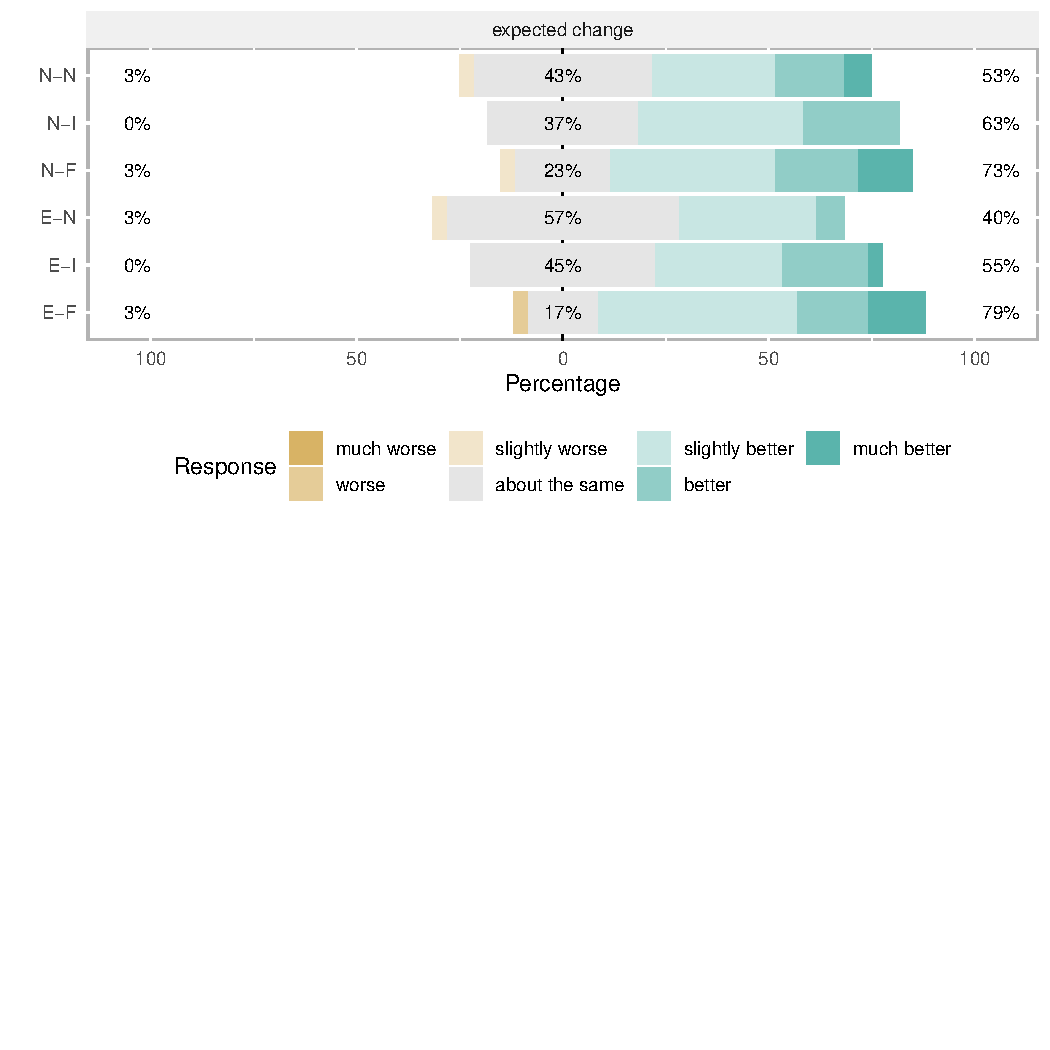
\includegraphics[width=\linewidth]{2020_chi_explanation/figures/exp-plots-study1.pdf}
    \caption{Study 1 participant responses for the subjective expected
change measure by condition. Participants expected
the model to improve. (Figure~\ref{fig:study1measures} describes $y$-axis labels.)}
    \label{fig:study1exp}
\end{figure}

\textbf{Feature-level feedback increased expected improvement compared to no feedback}.
%
\textit{Feedback} significantly increased users' expectations ($F_{2,172}=5.29, p=.006$);  post-hoc comparisons showed that feature-level feedback raised expected improvement compared to no feedback ($p<.05$), partially supporting \textbf{H2.1}. The main effect of \textit{Explanation} was not significant ($F_{1,172}=1.28, p=.259$; opposing \textbf{H2.2}), nor was the \textit{Explanation} $\times$ \textit{Feedback} interaction ($F_{2,172}=.42, p=.656$).

\textbf{A substantial portion of participants expected model corrections, even without feedback}.
%
Across all three feedback conditions, about half or more of participants expected the model to improve (rating > 4): 76.3\% of 59 who had feature-level feedback, 59.3\% of 59 who had instance-level feedback, and even $47\%$ of 60 who had no feedback. 

%Confirming our rating scale data, of the 118 participants who provided feedback, more expected model improvement after giving feature-level feedback (45 of 59) than those that provided instance-level feedback (35 of 59).
%Of the 60 participants who did not provide feedback, $53\%$ (of 30) who did not receive an explanation and $40\%$ (of 30) who did thought the model would improve. Suggesting that explanations tempered expected improvement in the no feedback condition.

%After the interaction phase, participants predicted how the model would ``now'' label emails that were the same as or similar to emails in the original set of 20. 
Participants' predictions about how what the model would do with the four same/similar ``evaluation'' emails  reflected this strong expectation of improvement. 
%, resulting in 712 \textit{simulated model predictions}. 
For the previously correct emails, participants thought the model would now be incorrect in only 4 of 712 instances, and each of these was for a ``similar'' email rather than the email that was exactly the ``same'' as in the initial set of 20.

For the previously incorrect emails, ``similar'' and ``same'' follow a similar pattern, so we focus on the ``same'' email to provide a straightforward assessment of whether participants think the model will improve. 
%
Most (82\%) of participants who provided feedback ($N=118$) thought the model would get the previously incorrect email correct (Table~\ref{tab:study1eval}), which is not surprising given that they had spent time trying to improve the model.
%
More surprising, however, is that 53\% of  participants in the no feedback condition ($N=60$) thought the model would somehow correct itself. %As with the subjective rating scale data, Table~\ref{tab:study1eval} shows that the influence of explanations on this expectation for improvement is, if anything, unclear.

\begin{table}[t]
    \centering
    \begin{tabular}{cccc}
    \toprule
              & \multicolumn{3}{c}{{\bf Feedback}} \\
              \cline{2-4}
        {\bf Explanation} & None & Instance & Feature \\
         \midrule
        None & 63\% & 80\% & 90\% \\
        Feature & 43\% & 86\% & 73\% \\
        \bottomrule
    \end{tabular}
    \caption{Percentage of Study 1 participants (\textit{N}=178) by condition during the ``evaluation phase'' who thought the model would now correctly label an email it had previously labeled incorrectly. Many participants in the \textit{no feedback} conditions thought the model would self correct.}
    \label{tab:study1eval}
    \vspace{-15pt}
\end{table}

\textbf{Participants described the model improving from their feedback or learning from its mistakes}.
We coded participants open-ended reasons for their expected change ratings, resulting in nine codes. Participants felt the model would improve with ``feedback'' ($29\%$), was capable of ``self learning'' ($20\%$), was ``high quality'' ($5\%$), or showed ``evidence of improvement'' ($1\%$). 
%
Those who felt it would not improve cited that it received ``inadequate feedback'' ($14\%$), showed ``no evidence of improvement'' ($11\%$), had ``nothing to learn from'' ($6\%$) or was of ``low quality'' ($5\%$). And, $9\%$ of participants gave ``other'' reasons.
%
%Many participants expected the model to improve from the ``feedback'' they provided (29\% of all 178 participants) or that it would \textit{self correct} (i.e., model ``self learning'' from its mistakes) (20\%). 

Interestingly, of the 60 participants who did not provide feedback (-N), 17 (28\%) still expected the model to learn from its mistakes, such as,  \textit{``it would take what it did wrong, learn from it, and apply it in future trials''} (LP141, N-N), or reported other misconceptions, including, \textit{``these programs get better as they function and learn algorithms''} (LP154, E-N). 
%
In fact, only 13\% of the 60 participants who did not provide feedback \textit{correctly} identified that the model would not improve as it had ``nothing to learn from'', like, \textit{``if it still used the same words to try to identify the correct sports emails, then it would still make the same amount of errors''} (LP87, E-N).

%Twenty-one participants (12\%) thought they provided ``inadequate feedback'', or not enough (quality or quantity) to improve the model. \lkf{is the rest of this para interesting or can we cut it}10 of these gave instance-level feedback (6 provided feature-level and 5 provided no feedback) and suggested the model needed additional information beyond just labels, such as keywords. For example, LP60 (E-I) said, \textit{``It would have been better if I'd had the option to tell it when it should have looked at different keywords''}, while LP72 (E-I) said, \textit{``I don't know what it learned, because I wasn't able to provide detailed feedback''}.
%Of the 21 participants who thought the system was given ``inadequate feedback, 10 gave instance-level feedback and suggested the model needed additional information beyond just labels, such as keywords. For example, LP60 (E-I) said, \textit{``It would have been better if I'd had the option to tell it when it should have looked at different keywords''}, while LP72 (E-I) said, \textit{``I don't know what it learned, because I wasn't able to provide detailed feedback''}. 

%Finally, some participants were not sure if the model would improve as there was ``no evidence of improvement'' during the interaction phase. $11\%$ of all participants suggested this, and surprisingly, $15\%$ of the 118 participants who gave feedback reported this, even though we explicitly reminded those participants that the model would not update with their feedback until after the interaction phase.\lkf{this last sentence is similar to the findings already reported in the prev improvement section, again suggesting to me that you should put this qual stuff up there and shorten it}

\textbf{Feature-level feedback reduced perceived accuracy compared to no feedback}.
%
\lkf{this is weird and needs to be touched on in Discussion}
Overall, participants thought the system worked fairly well, giving it an average accuracy rating across all conditions of 5.2 out of 7 ($SD=1.1$).
However, counter to our other user experience measures, feature-level feedback had a negative effect on perceived accuracy. There was a significant main effect of \textit{Feedback} on perceived accuracy ($F_{2,172}=4.72, p=.010$), with posthoc pairwise comparisons showing that feature-level feedback reduced perceived accuracy compared to no feedback ($p<.05$). Neither the main effect of \textit{Explanation} nor the \textit{Explanation} $\times$ \textit{Feedback} interaction effect were significant (respectively: $F_{1,172}=1.59, p=.209$; $F_{2,172}=2.20, p=.114$). 

\subsubsection{Quality of and Desire for User Feedback}
% three points: users want to provide feedback, how good is their feedback for the model, and how do users 'features' compare to the model's 'features'
Participants thought being able to provide feedback was important ($M=6.4$ out of 7, $SD=.9$), regardless of condition~(Figure~\ref{fig:study1measures}); there were no significant main or interaction effects on this measure. However, do the experimental conditions impact feedback \textit{quality}? To answer this question, we applied participants' feedback to the model after the study.

\textbf{Feedback improved the model, regardless of explanation}.
%, and explanation does not appear to impact this improvement}.
We incorporated instance-level feedback by including the 20 emails labeled by the participant as additional training emails. To incorporate the feature-level feedback, we adjusted the classifier's weight for each word provided by the participant: the word weight was both increased by 20\% for the specified class and decreased by 20\% for the opposite class.\lkf{seems arbitrary... anything we can cite here a way we can justify?}\amr{agreed... Ron or Melissa?}\jbg{If it was $\beta_a \rightarrow \frac{\beta_a + \alpha_a}{\sum \beta_\cdot + \alpha_a}$, then you can phrase it as increasing the Dirichlet prior with a $\beta$ pseudocount (i.e., the user provided an additional training example with weight $\alpha$; this is how Settles justified it).}
%This resulted in $59$ feature-updated models and $59$ instance-updated models.

The feature-updated models were 86.2\% accurate on average ($SD=2.7\%$), which is a 9.7 percentage point improvement over the initial low quality model.
In comparison, the instance-updated models were 83.6\% accurate ($SD=1.4\%$)---a 7.1 percentage point improvement. Instance and feature model improvements were similar regardless of whether the participants saw an explanation (difference in accuracy $<.2\%$).

\textbf{Participants did not agree with the words the model thought were important}.
The 59 participants who gave feature-level feedback highlighted a total of $3,533$ words. Regardless of whether explanations were shown or not, we compared the model's top three words for each email (i.e., the words the model would have highlighted) to the three words selected by the participant. Most (76.9\%) of the participants' words were not in the model's top set. This disagreement is likely due both to the model's low quality and because the explanation method can highlight words that are probable for the non-predicted class (see Limitations). Participants with explanations were more likely to reuse the model's words (28\% of selected words overlapped with the model's) than the 30 participants who did not see explanations (21\%).  

\subsection{Summary}
Explanations significantly increased frustration, while feedback---especially feature-level---significantly decreased it (partial support for \textbf{H1.1} and \textbf{H1.2}). There were similar patterns for other user satisfaction measures (trust and acceptance). Therefore, the worst combination was explanation without feedback, and the best was no explanation with feedback. Open-ended responses suggested that frustration was primarily due to the low model quality exposed by explanations and \textit{not} inability to provide feedback, as we had hypothesized. Although ability to provide feedback did temper some of the frustration. This general dislike for explanations confirms prior work where user perceptions were negatively impacted by explanations that exposed flaws and limitations~\cite{Cai2019TheInterface}. While this may seem inconsistent with our hypothesis at first blush, an alternate interpretation is that explanations can improve satisfaction \emph{so long as users have a means for feedback}. 

Feedback also significantly increased expectations of model improvement, as hypothesized in \textbf{H2.1}, but particularly for feature-level feedback opposed to none. Explanation did not impact expected change, in contrast to \textbf{H2.2}.
Also, somewhat surprisingly, participants  expected the model to improve; including many who had not provided feedback. %We discuss this and general misconceptions regarding ML models in the Discussion.

\section{Study 2: Understanding Explanations and Feedback with a High Quality Model}
%
In Study~1, expectations rose with feedback but not explanations and satisfaction fell with explanations but rose with feedback.
%
As the Study~1 model's low quality appeared to overwhelm participants' subjective ratings, an additional study had a higher quality model. While we expected participants to be more satisfied with the higher quality model (e.g., observed and stated model accuracy can affect users' trust~\cite{Yin2019UnderstandingModels}), we retained the Study~1 hypotheses regarding our primary measures (frustration and expected change).

\subsection{Method}
This experiment was exactly the same as Study~1 with the exceptions described here. We trained the \texttt{MultinomialNB} classifier on $200$ labeled training emails ($100$ from each class), with $94.4\%$ accuracy on the test set. This model predicted the correct label for $18$ of the $20$ emails in the interaction phase. As in Study~1, we chose four emails for the evaluation phase (two ``same'' and two ``similar''), but because of the higher accuracy of the model in Study~2 there were no available emails that were ``similar'' to ones the model labeled incorrectly in the evaluation phase; thus, both of the ``similar'' emails were similar to previously correct ones. 

As in Study~1, we recruited $180$ participants ($99$ female, $78$ male, $3$ unspecified). Two participants were aged 18--24 years old, 46 aged 25--34, 66 aged 35--44, 43 aged 45--54, 16 aged 55--64, and 6 aged 65--74. Participants had varied prior knowledge of machine learning (63 participants had none, 65 had a little, 50 had some, two had a lot, and none had expert), hockey (23 had none, 64 had a little, 58 had some, 25 had a lot, and none had expert), and baseball (12 had none, 37 had a little, 66 had some, 54 had a lot, and 11 had expert).

Study sessions took on average $22.8$ minutes ($SD=14.6$), and we used the same measures and data analyses as in Study~1. Our dataset included all 180 participants. We used the Study~1 codes to code the open-ended responses for frustration and expected change. We refer to participants as HP1--HP180.

\newcommand{\FigureHighMeasure}{
\begin{figure}[t]
    \centering
    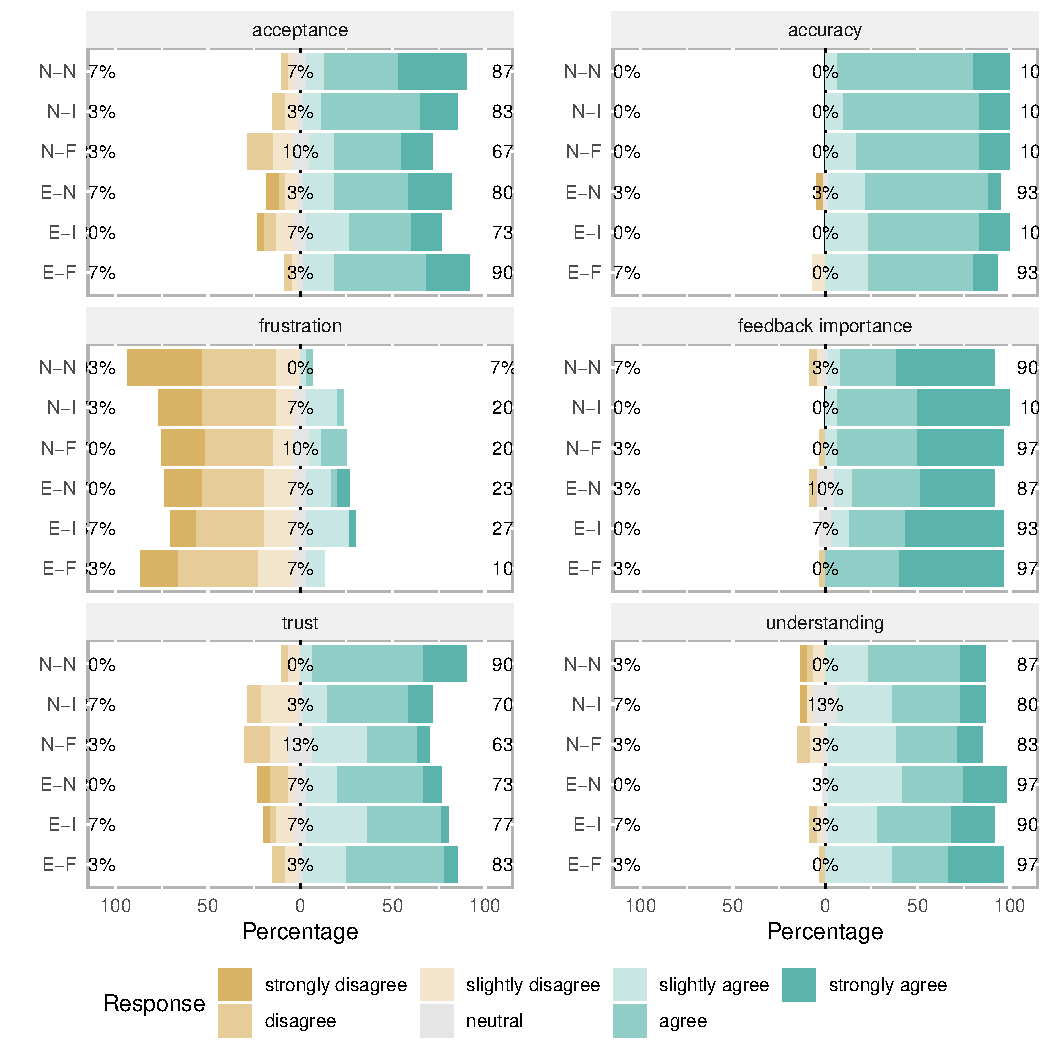
\includegraphics[width=.48\textwidth]{figures/study2-measures.pdf}
    \caption{Study 2 responses by condition for the main subjective measures (except expected change). Participants were more satisfied, but trust suggests nuance (e.g., E-N vs. N-N, without feedback, explanation has a negative impact).
    %on seven-point  scales from ``strongly disagree'' to ``strongly agree.'' 
    (Figure~\ref{fig:study1measures} describes $y$-axis labels.)}
    \label{fig:study2measures}
    \vspace{-10pt}
\end{figure}
}

\newcommand{\FigureHighExp}{
\begin{figure}[t]
    \centering
    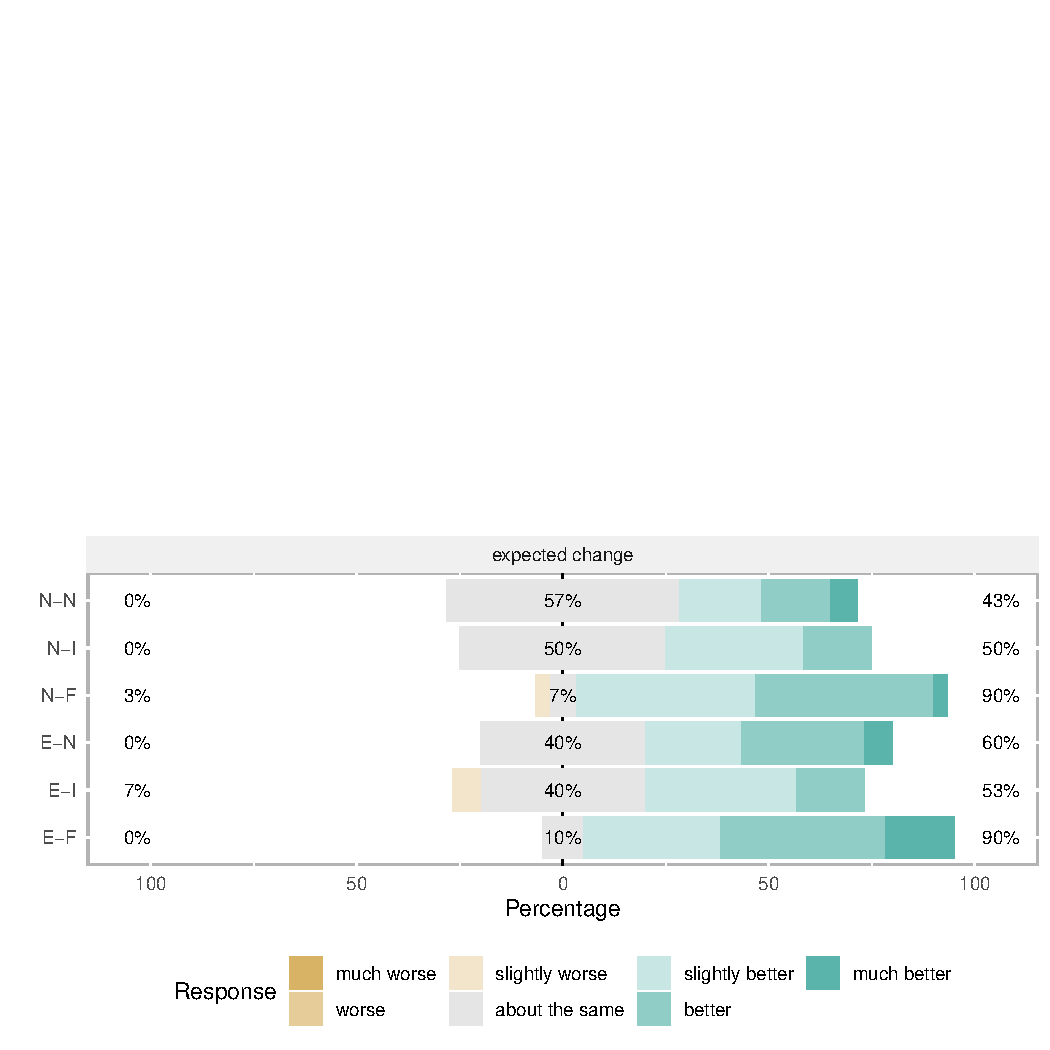
\includegraphics[width=.48\textwidth]{figures/exp-plots-study2.pdf}
    \caption{Study 2 responses for the expected change measure by condition, showing that in general participants expected improvements (green bars), but more in feature-level feedback conditions (E-F and N-F). (See Figure~\ref{fig:study1measures} for a description of y-axis labels).}
    \label{fig:study2exp}
    \vspace{-10pt}
\end{figure}
}
\FigureHighMeasure

\subsection{Results}
Figure~\ref{fig:study2measures} and \ref{fig:study2exp} show the rating responses for the seven main subjective measures by condition.
% satisfaction
Overall, participants were less frustrated with the high quality model than the low quality one (Figure~\ref{fig:study1measures}). 
%
The interaction between explanation and feedback was significant for other subjective measures: trust and acceptance. 
% expected improvement & feedback ability
As in Study~1, feedback impacted expected change but explanation did not, and participants expected the model to improve and wanted the ability to provide feedback.

Regarding task difficulty, participants again performed well: 92\% of their 3,600 answers to us were correct, while 7\% were ``not sure'' and only 1\% were incorrect. 
%
We provide detailed results regarding satisfaction, expectations and perceptions, and quality and desire for feedback in the following sections.


\subsubsection{User Satisfaction}
%
Overall, frustration was lower ($M=2.64$ of 7, $SD=1.54$) compared to the low quality model in Study 1 ($M=3.90$, $SD=1.85$). Perhaps accordingly, there were no significant main or interaction effects on frustration. Open-ended responses suggest explanations exposed the high quality model's \textit{good} behavior.
%
Trust and acceptance ratings were also relatively high compared to Study 1: 5.1 out of 7 on average for trust ($SD=1.5$) and 5.4 for acceptance ($SD=1.5$) here compared to 4.1 for trust ($SD=1.7$) and 4.3 for acceptance ($SD=1.9$) in Study 1. The interaction between explanations and feedback on these measures was significant.

\textbf{Trust and acceptance were affected by the combination of explanations and feedback}.
%
Neither explanation nor feedback had a clear effect on trust; the main effects of \textit{Feedback} ($F_{2,174}=2.59, p=.078$) and \textit{Explanation} ($F_{1,174}=2.00, p=.159$) were not significant. However, the interaction between \textit{Explanation} and \textit{Feedback} was significant ($F_{2,174}=5.69, p=.004$), meaning that certain combinations of explanations and feedback impact trust. 

From the responses (Figure~\ref{fig:study2measures}), when feature-level feedback is requested, not providing an explanation might decrease trust (N-N compared to N-F). And, without feedback, explanation might decrease trust (N-N compared to E-N). After a Holm-Bonferroni correction, only the former posthoc pairwise comparison was significant: participants trusted the model more with neither feedback nor explanation compared to a model with feedback but no explanation ($p < .05$). 

Acceptance shows a similar pattern: while there is no clear effect of either explanation or feedback, some combinations do; the \textit{Explanation} $\times$ \textit{Feedback} interaction was significant ($F_{2,174}=4.11, p=.018$), while the main effects of \textit{Feedback} ($F_{2,174}=1.23, p=.295$) and \textit{Explanation} ($F_{1,174}=.036, p=.850$) were not. While Figure~\ref{fig:study2measures} shows similar trends for acceptance as for trust, no posthoc pairwise comparisons were significant after a Bonferroni correction, so further work is needed to explore this relationship.

\FigureHighExp


% why frustrated
\textbf{Explanations may have shown participants that the model was behaving properly.}
%
Participants gave lower frustration ratings than in Study~1 (Figure~\ref{fig:study2exp}); users said the model was ``good enough'' (49\% of all participants) or would ``save time'' (23\%). Only 15\% of participants felt the model was ``not good enough'', that is, not of an acceptable accuracy for the task. 

In Study~1, explanations exposed issues with the model's highlighted words, resulting in 81\% of the 89 participants who had received explanations in that study thinking the model was ``not good enough.'' Study~2 responses were the opposite: 80\% (of 90) participants who saw explanations thought the model was ``good enough'', and  explicitly described good model behavior, such as \textit{``\dots I was able to see the reasoning from the machine and I agreed with it most of the time''} (HP139, E-F). For Study~2 participants who did not see explanations, only 65\% (of 90) felt the model was ``good enough'', emphasizing how explanations can improve perceptions of model quality with a higher quality model. 

% I think the below is interesting, but we already have a TON of results
%Some of the responses expose differences in what participants consider to be an acceptable accuracy, particularly as it relates to frustration. For example, HP17 (N-F) gave a low frustration rating and said, \textit{``I think it does a really good job. 90ish percent is great,''} whereas HP71 (E-N) said he or she would be frustrated, \textit{``because it wasn't 100\% correct.''} HP5 (E-N) said, \textit{``[...] if I were going to trust this model to the point where I was responsible for what it was doing, I would want almost perfect accuracy [...] I wouldn't be frustrated, though.''} These responses provide some intuition into why \textit{Explanation} and \textit{Feedback} did not impact frustration scores for the high quality model.

\subsubsection{User Expectations for and Perceptions of the Model}
% four points: expected improvement, why, perceived accuracy and perceived understanding
Figure~\ref{fig:study2measures} and \ref{fig:study2exp} show responses for subjective rating scales regarding expectations and perceptions of the model. On average, participants expected improvement ($M=5.0$, $SD=1.0$), thought they understood the model ($M=5.5$, $SD=1.2$), and thought it worked well ($M=5.9$, $SD=.76$).

As detailed below, feature-level feedback caused participants to think the model would improve, and explanation yielded higher perceived understanding. Neither explanation nor feedback had an impact on perceived accuracy. Open-ended responses suggest misconceptions regarding how ML models evolve, providing further explanation for why a substantial portion of participants, regardless of condition, expected the model to improve (Figure~\ref{fig:study2exp}).\footnote{We do not report on participants' simulated model predictions due to space and because trends are in line with the rating data.}  

\textbf{Feature-level feedback increased expected improvement}.
%
As in Study~1, \textit{Feedback} significantly impacted expected change ($F_{2,174}=15.84, p < .001$). Posthoc pairwise comparisons showed that feature-level feedback resulted in higher expected improvement than instance feedback or none (both comparisons $p<.05$). \textit{Explanation} did not have a significant impact on expected change ($F_{1,174}=.79, p=.375$) nor did the \textit{Explanation} $\times$ \textit{Feedback} interaction ($F_{2,174}=1.41, p=.246$).

%\textbf{Participants may still expect correction, but less so when the model is higher quality}.
%
%\lkf{this para really really needs some descriptive stats... in general, one limitation of your results section currently is that it's mostly about p values and descriptives (that people can actually understand) are not mentioned much and instead people have to read the graphs... this example here is perhaps one of the more obvious ones that needs to be fixed though}
%Table~\ref{tab:study2eval} shows the percentage of participants who thought the model would correctly label a previously incorrect email in the evaluation phase.

%\begin{table}[t]
%    \centering
%        \begin{tabular}{cccc}
%    \toprule
%              & \multicolumn{3}{c}{{\bf Feedback}} \\
%              \cline{2-4}
%        {\bf Explanation} & None & Instance & Feature \\
%         \midrule
%        Without & 50\% & 53\% & 57\% \\
%        With &47\% & 57\% & 80\% \\
%        \bottomrule
%    \end{tabular}
%    \caption{Percentage of Study 2 participants ($N=180$) in the different conditions who thought the model would correctly label a previously incorrectly labeled email. Those who did not provide feedback, therefore, thought the model would self correct.}
%    \label{tab:study2eval}
%\end{table}

% why expectations?
\textbf{Participants described misconceptions for how ML changes over time}.
%
Participants gave similar reasons for expecting model change as in Study~1. 27\% of all participants credited the ``feedback'' they provided while 19\% suggested the model was ``self learning.'' Many participants noted similar misconceptions, including, \textit{``my understanding is these sorts of things just get better at what they do the more they do them''} (HP84, E-N) and,
%\textit{``The model is programmed to automatically update its system with corrections and new information''} (HP111, N-N),
 \textit{``it learns with each new experience, and I choose the word `experience' intentionally as the machine gains consciousness''} (HP62, N-I).

% can maybe cut the below, but I do come back to it in the discussion..
Similar to Study~1, 21 (12\%) participants thought their feedback was ``inadequate'' (whether in quality or quantity). Of these, 17 provided instance-level feedback (compared to three who provided no feedback and three who provided feature-level feedback), and suggested that they would have preferred to tell the model \textit{why} it was wrong. 
%HP3 (N-I) said, \textit{``I'm not really sure that it learned anything because of the fact that I didn't explain why it was wrong}, %Maybe it can, but I don't really think so''
For example, HP128 (E-I) said, \textit{``simply telling it that it was wrong may make it less accurate, but it is unlikely to make it more accurate without knowing how it made its mistake.''}

% perceived understanding
\textbf{Explanations increased perceived understanding}.
%
\textit{Explanation} significantly impacted perceived understanding ($F_{1,174}=3.92, p-0.49$). Participants thought they understood the model more when given an explanation (Figure~\ref{fig:study2measures}). Neither the main effect of \textit{Feedback} ($F_{2,174}=.13, p=.876$) nor the \textit{Explanation} $\times$ \textit{Feedback} interaction effect were significant ($F_{2,174}=.53, p=.591$).

\subsubsection{Quality and Desire for User Feedback}
Like in Study~1, participants wanted the ability to provide feedback ($M=6.3$ of 7, $SD=1.0$), regardless of condition (Figure~\ref{fig:study2measures}). There were no significant main or interaction effects on this measure. But how useful is their feedback for the high quality model?

% improvement from feedback
\textbf{Feedback provided only minor improvement}.
%
%Incorporating the Study 2 feedback into the initial, high quality model, resulted in $60$ feature updated models and $60$ instance updated models. 
We incorporated participant's feature-level and instance-level feedback into the model.
While the updated models in Study~1 greatly improved, in Study~2 they did not. The feature updated models averaged 95.8\% accuracy ($SD=.8\%$), only a 1.4 percentage point improvement over the initial high quality model.
The instance updated models had 95.1\% accuracy ($SD=.5\%$; a .7 percentage point improvement). As in Study~1, instance and feature model improvements were similar regardless of whether the participants saw an explanation (difference in accuracy $<.2$).

% feature-level feedback model agreement
\textbf{Participants agreed more with the high quality model's words}.
%
Participants provided 3,589 words as feature-level feedback. Participants were similarly likely to provide new words~(1,942) as reuse model words~(1,647), unlike Study~1 participants who reused less than 25\% of the model's words. 
The 30 participants shown explanations reused provided words (51.6\% overlap of their words to the model's important words), more than the 30 who did not see explanations~(40.2\%). %We saw the opposite effect in Study~1 (there participants used less model words but more when given explanations).

\subsection{Summary}
%
Neither feedback nor explanation impacted frustration, which was generally lower than in Study~1.
For other user experience measures, there were no main effects either, although significant interaction effects on trust and acceptance suggest nuance in how explanations and feedback impact each other.
%
As with the low quality model, feature feedback significantly increased expected change, this time over both instance and no feedback (confirming partial support for \textbf{H2.1}), but explanation did not have an effect. Again, participants generally thought the model would improve. 


%Overall, frustration was lower ($M=2.64$, $SD=1.54$) compared to the low quality model ($M=3.90$, $SD=1.85$). 
%feature-level feedback without explanation significantly reduced trust in the model compared to simply having no explanation and no feedback. We find some evidence that trust decreases when explanations are provided without support for feedback\lkf{please don't add more stats in the summary and discussion... here we are supposed to be making things super easy to read and highlighting the interesting takeaways} ($M=4.97$, $SD=1.77$) compared to no explanations without feedback ($M=5.83$, $SD=1.21$). Further work is needed to explore these interactions. 

%: 48\% of the 60 who did not provide feedback and 62\% of the 120 who provided feedback thought the model would get a previously incorrect email correct. 

%We find some evidence that trust decreases when explanations are provided without support for feedback ($M=4.97$, $SD=1.77$) compared to no explanations without feedback ($M=5.83$, $SD=1.21$).
%\section{Discussion and Related Work}
\label{sec:discussion}

We connect the improvements made by conformity \loo{} to 
model confidence issues, compare alternative interpretation improvements,
and discuss further features of \dknn{}.

\subsection{Issues in Neural Network Confidence}
\label{sec:overconfidence}

Many existing feature attribution methods rely on estimates
of model uncertainty: both input gradient and confidence \loo{} rely on
prediction confidence, our method relies on \dknn{} conformity.
Interpretation quality is thus determined by reliable uncertainty estimation. 
For instance, past work shows relying on neural network confidence
can lead to unreasonable interpretations~\cite{kindermans2017unreliability,
ghorbani2017interpretation, feng2018rawr}. Independent of interpretability,
\citet{guo2017calibration} show that neural network confidence is unreasonably
high: on held-out examples, it far exceeds empirical accuracy.
This is further exemplified by the high confidence predictions produced on
inputs that are adversarial~\cite{szegedy2013intriguing} or contain solely
noise~\cite{goodfellow2014explaining}.

\subsection{Confidence Calibration is Insufficient}

We attribute one interpretation failure to neural network
confidence issues. \citet{guo2017calibration} study
overconfidence and propose a calibration procedure using
Platt scaling, which adjusts the temperature parameter of the softmax
function to align confidence with accuracy on a held-out dataset.
However, this is not input dependent---the confidence is lower
for both full-length examples and ones with words left out. 
Hence, selecting influential words will remain difficult.

To verify this, we create an interpretation baseline using temperature 
scaling.
The results corroborate the intuition: calibrating the confidence 
of \loo{} does not improve interpretations. Qualitatively, the 
calibrated interpretation results remain comparable to  
confidence \loo{}. Furthermore, calibrating the \dknn{}
 conformity score as in \citet{papernot2018dknn} did not improve
interpretability compared to the uncalibrated conformity score.

\subsection{Alternative Interpretation Improvements}

Recent work improves interpretation methods through other
means. \citet{smilkov2017smoothgrad} and \citet{sundararajan2017axiomatic}
both aggregate gradient values over multiple
backpropagation passes to eliminate local noise or satisfy
interpretation axioms. This work does not address 
model confidence and is orthogonal to our \dknn{} approach. 
 
\subsection{Interpretation Through Data Selection}

Retrieval-Augmented Convolutional Neural Networks~\cite{zhao2018retrieval} are similar
to \dknn{}: they augment model predictions with an information
retrieval system that searches over network activations from the training data. 

Retrieval-Augmented models and \dknn{} can both select influential
training examples for a test prediction. In particular, the
training data activations which are closest to the test point's 
activations are influential according to the
model. These training examples
can provide interpretations as a form of analogy~\cite{caruana1999casebased}, an
intuitive explanation for both machine learning experts and non-experts~\cite{klein1989biases,
kim2014bayesian,
koh2017influence, wallace2018trick}. However, unlike in computer vision where
training data selection using \dknn{} yielded interpretable examples~\cite{papernot2018dknn},
our experiments did not find human interpretable data points for \abr{sst} or
\abr{snli}. 
  		
\subsection{Trust in Model Predictions}

Model confidence is important for real-world
applications: it signals how much one should trust
a neural network's predictions. Unfortunately, users may be 
misled when a model outputs highly confident predictions on rubbish
examples~\cite{goodfellow2014explaining, nguyen2015fooled} or adversarial
examples~\cite{szegedy2013intriguing}. Recent work decides when
to trust a neural network model~\cite{ribeiro2016lime,
doshivelez2017towards, jiang2018trust}. For instance, analyzing local linear
model approximations~\cite{ribeiro2016lime} or flagging rare network activations
using kernel density estimation~\cite{jiang2018trust}. The \dknn{} conformity
score is a trust metric that helps defend against image adversarial
examples~\cite{papernot2018dknn}. Future work should study if this robustness
extends to interpretations. 

%\section{Conclusion}
\label{sec:conc}
We introduce the new problem of noun phrase annotation, which is a generalization of \nel{}. 
We find that introducing noun phrase annotation may be useful in downstream tasks such as question answering. 
However creating a dataset for noun phrase annotation is a difficult task. 
We counter this problem by developing a human-in-the-loop method to efficiently annotate questions and motivate experts to annotate questions by assisting them with studying and directing tournaments. 
To explore the difficulty of noun phrase annotation, we propose experiments that compare the performance of \nel{} and coreference linkers on our noun phrase annotation dataset. 
We additionally design experiments to compare entity linking with multiple configurations in order to determine how best to assist users when entity linking. 
We finally design experiments to determine the effect that noun phrase annotation has upon question answering; we do this by comparing the accuracy of QA models when replacing entities with their entry in the knowledge base. 
Our next steps are to proceed forward with data collection, and to run the experiments on the noun phrase dataset. 
%\section{Discussion \& Conclusion}

%We present two controlled experiments to understand how the combinations of explanation and feedback affect users' satisfaction and expectations of improvement of high and low quality ML models. We conclude that, for the simple models and task of our studies, when possible explanations and feedback should be provided together: (1) while explanations negatively impacted user satisfaction with the low quality model, they can show users how to fix models, and support for feedback had positive effects; and (2) for the higher accuracy model, requesting detailed feedback without explanations reduced trust.
%Additionally, regardless of model quality, feature-level feedback increased expectations that models would improve, yet users generally expected model correction, regardless of whether they provided feedback or received explanations. 

\section{Discussion}

%\subsection{Main Takeaways}

We relate our findings to prior work and provide design recommendations for interactive and explainable ML systems. 
%
We also discuss limitations and extensions to more complex tasks, models, explanations, and feedback mechanisms.
%. 
%Participants wanted the ability to provide feedback regardless of model quality, and in particular they wanted to provide more detailed feedback. 
%
%Explanations exposed models' strengths or weaknesses, so they reduced satisfaction for low quality models, particularly when feedback was not supported. 
%
%In high quality models, explanations importantly told participants \emph{what} feedback was needed.
%
%Finally, participants may have had preconceived notions of how these models can change over time, with or without feedback, so care is required to manage expectations. We reflect on each of these findings in turn. %We discuss these points in detail below. 

% users want to provide feedback
\textbf{Users want the opportunity to provide feedback, and in particular, provide more than just labels}. 
%
% And, the ability to provide feedback had positive impacts for the low quality models.
%
In both studies and all conditions, participants felt strongly that the \textit{opportunity} to provide feedback was important; however, this does not tell us how often or whether users will provide such feedback in practice. Although, successful commercial projects, such Common Voice,\footnote{https://voice.mozilla.org/en} exemplify that users might be willing to spend time improving models. 
%

Our studies provide additional evidence for how different levels of feedback impact user behavior and subjective response. In particular, we confirmed Amershi et al.'s~\cite{Amershi2014PowerLearning} recommendation that ``people naturally want to provide more than just data labels'' to ML models. 
%
With both the low and high quality models, only those participants who told the model what words were important (i.e., provided feature-level feedback) and not those who corrected or confirmed the model's predictions (i.e., instance-level), expected the model to improve more than participants in the no feedback condition. Similarly, some participants who provided instance-level feedback described their feedback as inadequate in open-ended responses.
%
Finally, not only was feature-level feedback better received by participants, for the low quality model it also improved accuracy more than instance-level feedback.
%; this difference was not seen for the high quality model. 
This ability of non-ML expert participants to improve the models in our study beyond just labeling data supports the goals of machine teaching~\cite{Wall2019UsingTeaching}.  


% in low quality models, feedback is good and explanations are bad, particularly if feedback is not provided
\textbf{Explanations can reveal model flaws, which users desire to fix}. 
Displaying uncertainty scores for model predictions negatively impacts users' perceptions~\cite{Lim2011InvestigatingApplications}; similarly, for the low quality model, explanations were frustrating, precisely because they exposed flaws, including \textit{uncertainty} in the model's reasoning.
Because feedback reduced frustration, the most frustrating combination of explanations and feedback for the low-quality model was thus a situation with explanations but no opportunity for feedback. Indeed, no explanations and no feedback may be the least frustrating design option; however, this combination would inherently limit the model's \textit{potential} performance, and likely result in disuse over time.
In such cases, explanations provide insight to how to solve model errors~\cite{Kulesza2015PrinciplesLearning}. Therefore, for similar models and tasks, when the model quality is low, feedback should be supported alongside explanations.

% in high quality models, feedback is good only if explanation is provided and explanations are particularly bad if feedback is not supported
\textbf{Explanations and feedback complement each other}.
%
For the high quality model, explanations increased understanding and may have exposed model strengths. But, models are rarely perfect, and participants wanted the opportunity to provide feedback to improve models. Therefore, providing explanations without means for feedback may reduce satisfaction. Future work should explore this relationship between explanations and feedback in more detail. 
%they can still have negative side effects if not employed with care. In our experiment, when feedback was not supported,  explanations appeared to reduce trust compared to no explanations. This aligns with our initial thinking that without feedback, explanations worsen user experience. Future work should explore this relationship in more detail. 
Feedback alone is not always positive either: asking participants for feature-level feedback without providing explanations reduced trust compared to when explanations were provided. Users may not want to provide detailed feedback without understanding why it is needed or how best to help the model. 
%
Therefore, to improve satisfaction, similar systems should neither request detailed feedback without explanation nor provide explanation without some means for feedback.

\textbf{Preconceived ML expectations should be managed}.
%\sherry{Be careful to not mislead users towards high expectation.}
%Finally, users may have preconceived notions of how these models can change over time, with or without feedback, so care is required to ensure expectations are managed. We discuss these points in detail below. 
Whether from prior experience or general misunderstanding, users may have misconceptions about whether and how much models can improve. In our experiments, many participants expected the model to improve regardless of whether they provided feedback. 
%
Open-ended responses provide insight: participants described their understanding that ML models  %\textit{``automatically update [...] with corrections and new information''} (HP111, N-N),
\textit{``get better as they function and learn algorithms''} (LP154, E-N), or even \textit{``gain consciousness''} (HP62, N-I).
%
%While more participants felt the low quality model had \textit{room for improvement} (about 25\%) than the high quality model (about 5\%), we see similar responses in both studies for expected improvement. This suggests that users may not fully understand to what extent these models are capable of improving.

Interactive ML designers must ensure that these expectations are managed, such as by clarifying how model feedback is treated or what accuracy the model could achieve. Or if feedback is not supported, designers should ensure users do not think they are in some way providing feedback to the model. %We discuss design constructs that may yield such feelings in the Future Work.


\subsection{Limitations \& Future Work}

\emph{Generalization from a tightly scoped domain.}
Our aforementioned findings are made in a tightly scoped domain, with a simple model and task (categorizing sports' emails). 
While this constrained setting provides a necessary first step in illustrating the relationship between explanations and feedback---it is simple enough to support a controlled experiment for non-expert users, and common enough in IML research to be compared to past studies---our findings should be generalized with caution. 
For example, explanations and feedback mechanisms in our studies were simple and intuitive. However, explanations in other domains, such as image classification, can be confusing or misleading~\cite{Adebayo2018SanityMaps}, and interaction with more complex models, such as topic models, exposes users to other challenges, such as instability and latency~\cite{Smith2018ClosingSystem}. These differences would likely affect satisfaction with and expectations of these systems. 
%

We hypothesize that even for more complex models or subjective tasks, 
%(e.g., recommender systems~\cite{Herlocker2000ExplainingRecommendations} or topic-model based document organization tools~\cite{Chaney2012VisualizingModels})
if users understand how models work and how they can better improve them, they will want the \textit{opportunity} to do so and may be frustrated if such feedback is restricted.
However, the \emph{degree} of their frustration would likely vary along with their actual desire and ability to provide feedback in more realistic settings. All are likely affected by  task and model complexity, task importance (and therefore user motivation), and domain expertise.
Would users be eager to provide feedback (in lieu of abandonment) in an imperfect self-driving car? Would they be less able to detect systems' mistakes for more subjective tasks?
Future studies should further explore the relationship between feedback and explanation. 
%Until then, we wish our observations that ``explanations and feedback should be provided together'' can encourage more cautious design of IML systems.


\emph{The effect of explanation and feedback mechanisms.}
Motivated by prior work~\cite{Narayanan2018HowExplanation, Kulesza2013TooModels}, our simple and truthful method chooses the top three overall important words for classification. 
This method inherently exposes system uncertainty in the low quality model, as words that are probable for both classes may be highlighted. This does not occur as often in the high quality model as it is more certain about most of the emails. Therefore, this could explain some of the additional frustration in the lower quality model.
Future work could explore the effects of different, more advanced, explanation types and feedback mechanisms.
For example, global explanations (e.g., differential explanations~\cite{Lakkaraju2019FaithfulModels}) might be equivalently faithful, while better counteracting the user experience concerns.
``Human-like'' explanations may increase expectations of improvement, as human-like characteristics in ML systems can cause users to believe systems will act rationally or take responsibility for their actions~\cite{Hook2000StepsReal}. 
Furthermore, explanations that expose when models are right for the wrong reason might further increase frustration if adequate feedback is not allowed, as users would be unable to rectify apparent mistakes.
For this case, to align the information received by the model and the user, feedback mechanisms should be changed accordingly.

\section{Conclusion}

We present two controlled experiments to understand how the combinations of explanation and feedback affect users' satisfaction and expectations of improvement of high and low quality ML models. We conclude that, for the simple models and task of our studies, when possible explanations and feedback should be provided together: (1) while explanations negatively impacted user satisfaction with the low quality model, they can show users how to fix models, and support for feedback had positive effects; and (2) for the higher accuracy model, requesting detailed feedback without explanations reduced trust.
%participants were less frustrated with the higher accuracy model; however, requesting detailed feedback without explanations reduced trust
%, and suggested similar patterns for providing explanations without feedback (compared to no explanation); (3) therefore, models should allow for feedback if explanations are provided; 
Additionally, regardless of model quality, feature-level feedback increased expectations that models would improve, yet users generally expected model correction, regardless of whether they provided feedback or received explanations.  


\section{Acknowledgments}
We thank the anonymous reviewers for their insightful and constructive
comments, and we thank Simone Stumpf and James Fogarty for their feedback on early ideas for this study. This work was partially supported by NSF Grants \abr{IIS}-1822494 and \abr{IIS}-1409287, ONR grant N00014-18-1-2193, the WRF/Cable Professorship, and the Allen Institute for Artificial Intelligence.
Any opinions, findings,
conclusions, or recommendations expressed here are those of the
authors and do not necessarily reflect the view of the sponsor.

\clearpage

% Balancing columns in a ref list is a bit of a pain because you
% either use a hack like flushend or balance, or manually insert
% a column break.  http://www.tex.ac.uk/cgi-bin/texfaq2html?label=balance
% multicols doesn't work because we're already in two-column mode,
% and flushend isn't awesome, so I choose balance.  See this
% for more info: http://cs.brown.edu/system/software/latex/doc/balance.pdf
%
% Note that in a perfect world balance wants to be in the first
% column of the last page.
%
% If balance doesn't work for you, you can remove that and
% hard-code a column break into the bbl file right before you
% submit:
%
% http://stackoverflow.com/questions/2149854/how-to-manually-equalize-columns-
% in-an-ieee-paper-if-using-bibtex
%
% Or, just remove \balance and give up on balancing the last page.
%\balance{}



% BALANCE COLUMNS
\balance{}

% REFERENCES FORMAT
% References must be the same font size as other body text.
\bibliographystyle{SIGCHI-Reference-Format}
\bibliography{bib/journal-full,bib/references,bib/bibliography}

\end{document}

%%% Local Variables:
%%% mode: latex
%%% TeX-master: t
%%% End:
